\documentclass{bioinfo}
\copyrightyear{2015} \pubyear{2015}

\access{Advance Access Publication Date: Day Month Year}
\appnotes{Manuscript Category}

\begin{document}
\firstpage{1}

\subtitle{Subject Section}

\title[PMMP]{A graph-based approach for modification site assignment in proteomics}
\author[Sample \textit{et~al}.]{Dafni Skiadopoulou\,$^{\text{\sfb 1,2}}$, Lukas Käll\,$^{\text{\sfb 3}}$, and Marc Vaudel\,$^{\text{\sfb 1,2,4,}*}$}
\address{$^{\text{\sf 1}}$Mohn Center for Diabetes Precision Medicine, Department of Clinical Sciences, University of Bergen, Bergen, Norway, and \\
$^{\text{\sf 2}}$Computational Biology Unit, Department of Informatics, University of Bergen, Bergen, Norway, \\
$^{\text{\sf 3}}$Science for Life Laboratory, School of Engineering Sciences in Chemistry, Biotechnology and Health, KTH Royal Institute of Technology, Stockholm, Sweden, and \\
$^{\text{\sf 4}}$Department of Genetics and Bioinformatics, Health Data and Digitalization,
Norwegian Institute of Public Health, Oslo, Norway.}

\corresp{$^\ast$To whom correspondence should be addressed.}

\history{Received on XXXXX; revised on XXXXX; accepted on XXXXX}

\editor{Associate Editor: XXXXXXX}

\abstract{\textbf{Summary:} 
	Assigning protein post-translational modifications to acceptor sites requires the distribution of modifications in a way that maximizes localization scores while avoiding chemically impossible configurations. We provide an efficient graph-based approach to this problem implemented both as standalone implementation and integrated in the PeptideShaker interface. \\
\textbf{Availability and Implementation:} 
	An open source implementation in Python is available at https://github.com/ProGenNo/peptides-modifications-matching under a GPL-3.0 license. An open source implementation in Java is available at github.com/compomics/compomics-utilities under an Apache-2.0 license. \\
\textbf{Contact:} \href{marc.vaudel@uib.no}{marc.vaudel@uib.no}\\
\textbf{Supplementary information:} Supplementary data are available at \textit{Bioinformatics}
online.}

\maketitle

\section{Introduction}

In mass spectrometry-based proteomics, mass spectra of fragmented peptides are matched against a database of protein sequences using a proteomic search engine, allowing the high throughput identification of peptide sequences together with their modification status (ref doi: 10.1038/nature01511). The localization of post-translational modifications (PTMs) on protein sequences is an important functional information (ref doi: 10.1002/elps.201200710). Furthermore, since amino acid substitutions can have the same mass difference as a modification, an incorrectly localized modification can be misinterpreted, yielding a false variant call (ref mass PTM variant). To evaluate the localization of modifications on a peptide sequence, multiple localization scores were developed that estimate the likelihood for a given acceptor site to be occupied for every modification of every peptide to spectrum match (PSM) (doi: 10.1074/mcp.R111.015305, 10.1002/pmic.201400372). 

Once the localization scores have been computed, the modifications are assigned to the sites of most likely localization before further processing, e.g. error rate estimation using Percolator (ref Percolator). It is important to note that due to differences in scoring, and especially since search engines often only consider the most intense peaks in mass spectra, the peptide maximizing the modification localization scores is not necessarily the best scoring peptide in the search engine results. And since the search engines also often have limitations in terms of how many modification sites combinations they consider, the peptide maximizing localization scores might not even be in the list of peptide candidates returned by the search engine.

In order to find the peptide maximizing the modification localization scores, the modifications found by the search engine need to be assigned to the site with highest localization score without yielding a configuration that is not chemically possible: modifications have different types of acceptor sites, e.g. amino acids or termini, and cannot be stacked on the same acceptor site. While maximizing the scores is trivial with a couple of modifications, e.g. phosphorylation and oxidation, the problem becomes more complex when combining many modifications with possible conflicting sites, e.g. in the study of histones (ref doi: 10.1021/cr500491u). Furthermore, since this needs to be conducted on millions PSMs per experiment, the site assignment needs to be fast.

Here, we propose a graph-based approach that models modifications and their acceptor sites, and returns a configuration that maximizes localization scores with controlled processing time. The modification assignment problem is reduced to the Maximum Weight Matching (MWM) problem in bipartite graphs, using modification localization scores as weights. We provide a standalone Python implementation as well as a Java implementation in the compomics-utilities library (ref doi: 10.1186/1471-2105-12-70) and demonstrate its usage in PeptideShaker (ref doi: 10.1038/nbt.3109).


\begin{methods}
\section{Methods}

\subsection{Graph modeling}

In this work the modification site localization problem is addressed by a graph theoretical approach. For each studied peptide a weighted bipartite graph ($G = \{V,E,w\}$) is used to model all possible combinations of modifications on the amino acid chain. In this graph we determine two kinds of vertices, the ones that represent the different modifications that have occured in the peptide (ie $D = \{d_1, d_2, \dots, d_k\}$) and the ones that represent all their possible acceptor sites in the amino acid chain (ie $A = \{a_1, a_2, \dots, a_n\}$). The set of the graph's vertices $V$ is then formed by the union of the sets $A$ and $D$ (ie $V = A \cup D$). For each modification, an edge is formed between the corresponding vertex and the ones that represent its possible acceptor sites. Moreover, a weight is assigned to each edge, taking the value of the confidence score (\textbf{is this really a confidence score???}, have to better describe the scores we're using...) which represents the probability of the modification to have occurred in that specific site of the amino acid chain. An example of a graph model for a modified peptide is presented in Fig. \ref{fig:PMMP_model}

Using this graph modeling we can reduce the modification site localization problem to the maximum weight matching problem on the resulting graph. This consists of finding a set of edges that are pairwise non-adjacent (without common vertices), in which the sum of weights is maximized. Solving this problem in the graph model of our application will result in the best combination of modifications localization on the peptide, based on their confidence scores. 

\begin{figure}[!tpb]%figure2
	\centerline{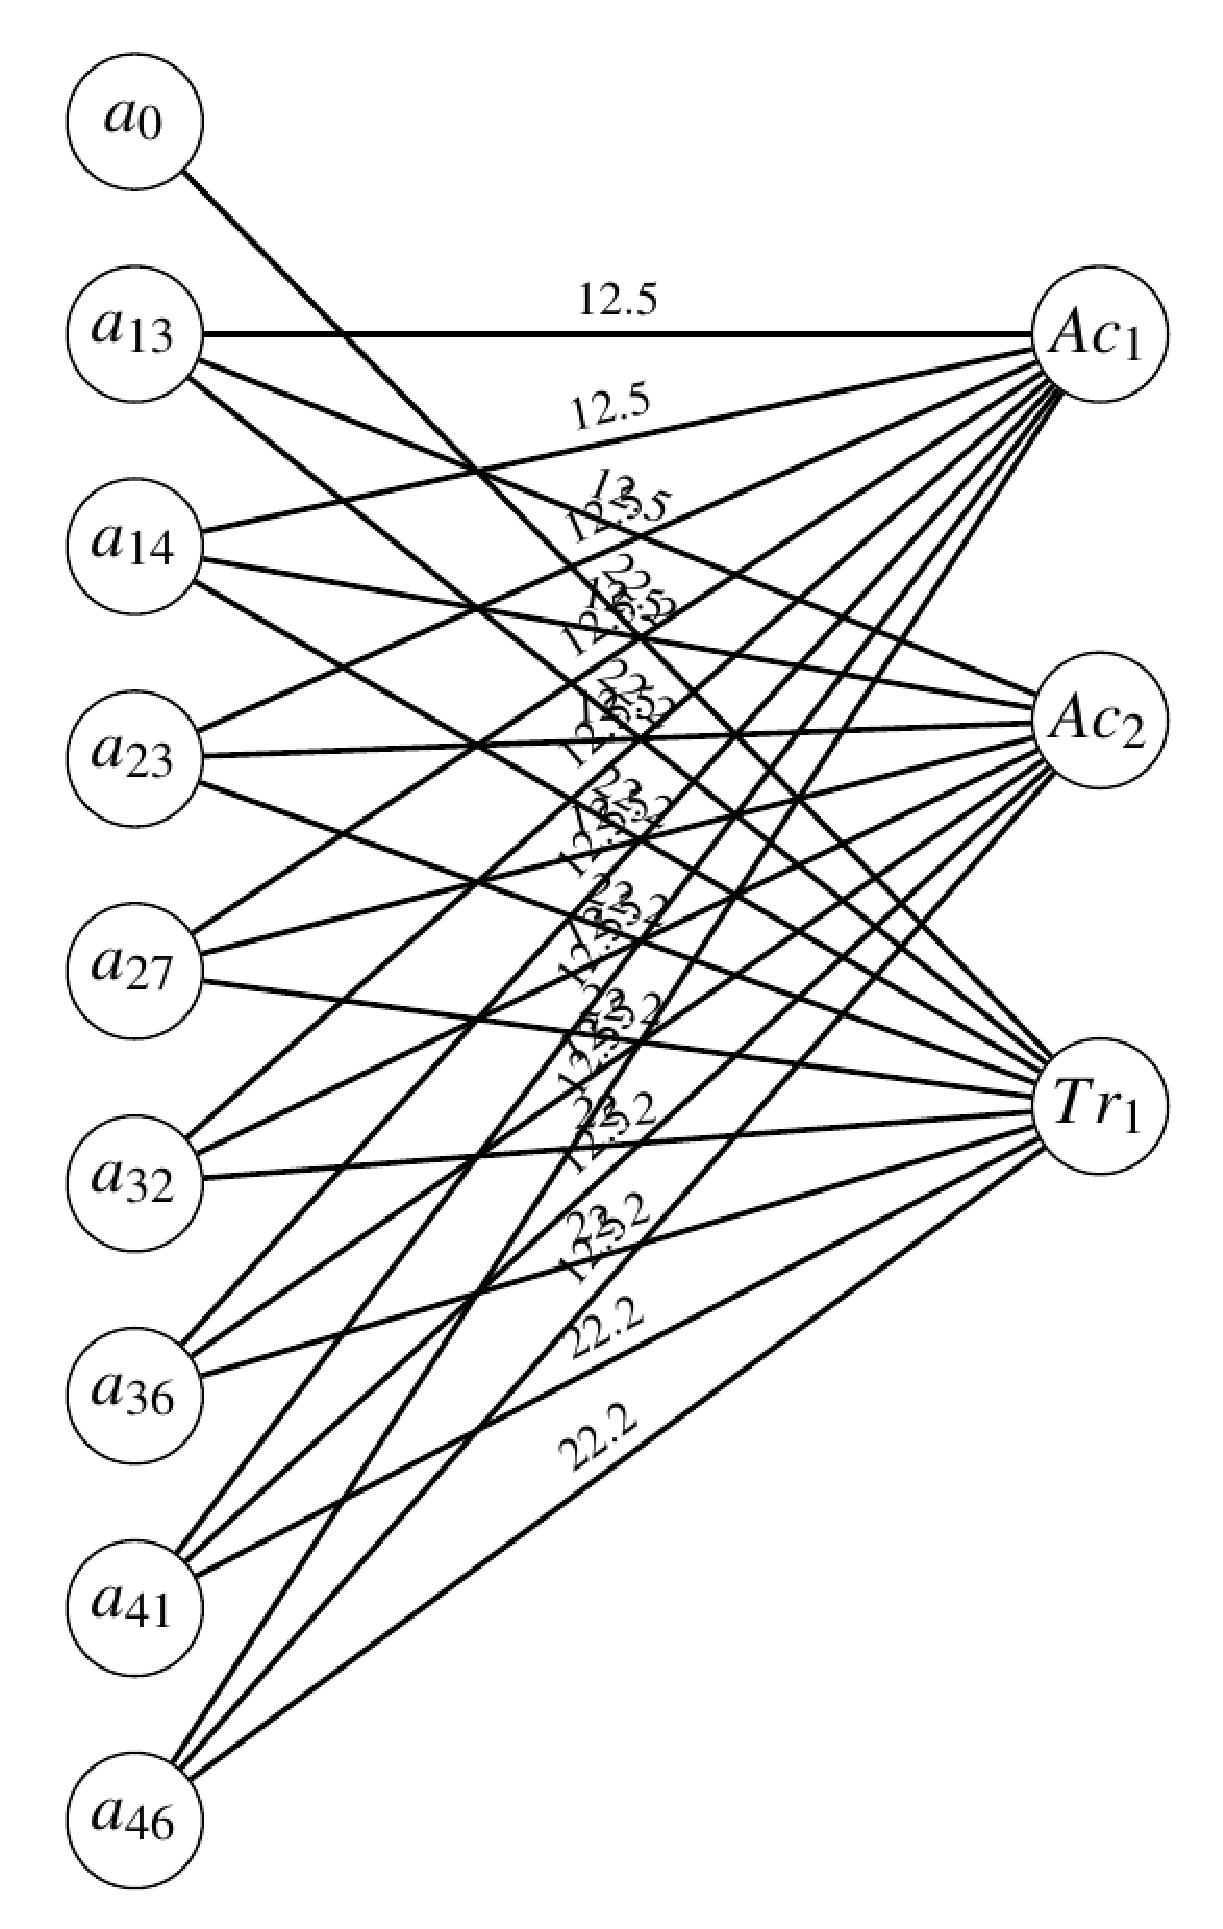
\includegraphics[width=0.2\textwidth]{pmmp_model.eps}}
	\caption{Graph representation of a peptide with 2 Acetylations and 1 Trimethylation with all their possible acceptor sites.}\label{fig:PMMP_model}
	%RLAVTGPRYRHPKKVGGTSPASKRTAKTALQKRPAKGGTSKRATQKTLA
\end{figure}

(mention the usage of python's networkX library implementation of the maximum weight matching algorithm based on methods invented by Jack Edmonds 1965 \textbf{???})

\subsection{Python implementation}

\subsection{Java implementation}

%text\vspace*{1pt}

%\begin{itemize}
%\item for bulleted list, use itemize
%\item for bulleted list, use itemize
%\item for bulleted list, use itemize\vspace*{1pt}
%\end{itemize}

%Text Text  Text Text Text Text Text Text\vadjust{\newpage}.

%\subsection{This is subheading}

%\subsubsection{This is subsubheading}


%\enlargethispage{6pt}

%\begin{table}[!t]
%\processtable{This is table caption\label{Tab:01}} {\begin{tabular}{@{}llll@{}}\toprule head1 &
%head2 & head3 & head4\\\midrule
%row1 & row1 & row1 & row1\\
%row2 & row2 & row2 & row2\\
%row3 & row3 & row3 & row3\\
%row4 & row4 & row4 & row4\\\botrule
%\end{tabular}}{This is a footnote}
%\end{table}

\end{methods}

%\begin{figure}[!tpb]%figure1
%\fboxsep=0pt\colorbox{gray}{\begin{minipage}[t]{235pt} \vbox to 100pt{\vfill\hbox to
%235pt{\hfill\fontsize{24pt}{24pt}\selectfont FPO\hfill}\vfill}
%\end{minipage}}
%\centerline{\includegraphics{fig01.eps}}
%\caption{Caption, caption.}\label{fig:01}
%\end{figure}

%\begin{figure}[!tpb]%figure2
%%\centerline{\includegraphics{fig02.eps}}
%\caption{Caption, caption.}\label{fig:02}
%\end{figure}


%\subsection{Test1}

\section{Results}

\subsection{Histone modification localization example}

\subsection{Performance}


%%%%%%%%%%%%%%%%%%%%%%%%%%%%%%%%%%%%%%%%%%%%%%%%%%%%%%%%%%%%%%%%%%%%%%%%%%%%%%%%%%%%%
%
%     please remove the " % " symbol from \centerline{\includegraphics{fig01.eps}}
%     as it may ignore the figures.
%
%%%%%%%%%%%%%%%%%%%%%%%%%%%%%%%%%%%%%%%%%%%%%%%%%%%%%%%%%%%%%%%%%%%%%%%%%%%%%%%%%%%%%%



\section{Conclusion}

%\begin{enumerate}
%\item this is item, use enumerate
%\item this is item, use enumerate
%\item this is item, use enumerate
%\end{enumerate}

%Figure~2\vphantom{\ref{fig:02}} shows\vadjust{\pagebreak} that the
%Text Text Text Text Text Text Text\break Text.

%Figure~2\vphantom{\ref{fig:02}} shows that the above method  Text
%Text Text Text\vspace*{-10pt}


\section*{Acknowledgements}


\section*{Funding}

This work was supported by the Research Council of Norway (project \#301178 to MV) and the University of Bergen.

This research was funded, in whole or in part, by the Research Council of Norway 301178. A CC BY or equivalent license is applied to any Author Accepted Manuscript (AAM) version arising from this submission, in accordance with the grant’s open access conditions.

%\bibliographystyle{natbib}
%\bibliographystyle{achemnat}
%\bibliographystyle{plainnat}
%\bibliographystyle{abbrv}
%\bibliographystyle{bioinformatics}
%
%\bibliographystyle{plain}
%
%\bibliography{Document}


\begin{thebibliography}{}

\bibitem[Yu {\it et~al}., 2020]{MSFragger}
Yu,F.T. {\it et~al}. (2020) Identification of modified peptides using localization-aware open search. {\it Nat Commun.}, {\bf 11} (1), 4065.

\bibitem[Yang {\it et~al}., 2018]{pSite}
Yang,H. {\it et~al}. (2018) pSite: Amino Acid Confidence Evaluation for Quality Control of De Novo Peptide Sequencing and Modification Site Localization {\it Journal of Proteome Research}, {\bf 17} (1), 119-128.

\bibitem[Baker {\it et~al}., 2011]{SLIP}
Baker,P.R. {\it et~al}. (2011) Modification site localization scoring integrated into a search engine.
{\it Mol. Cell. Proteomics.}, {\bf 10}, (M111. 008078)

\bibitem[Fermin {\it et~al}., 2013]{LuciPHOr}
Fermin,D. {\it et~al}. (2013) LuciPHOr: algorithm for phosphorylation site localization with false localization rate estimation using modified target-decoy approach. {\it Mol Cell Proteomics}, {\bf 12} (11), 3409-19.

\bibitem[Trudgian {\it et~al}., 2012]{ModLS}
Trudgian,D. {\it et~al}. (2012) ModLS: Post-translational modification localization scoring with automatic specificity expansion. {\it J. Proteomics Bioinform.}, {\bf 5}, 283–289.

\bibitem[Beausoleil {\it et~al}., 2006]{AScore}
Beausoleil,S.A. {\it et~al}. (2006) A probability-based approach for high-throughput protein phosphorylation analysis and site localization. {\it Nat. Biotechnol.}, {\bf 24}, 1285–1292.

\bibitem[Olsen {\it et~al}., 2006]{PTMScore}
Olsen,J.V. {\it et~al}. (2006) Global, in vivo, and site-specific phosphorylation dynamics in signaling networks. {\it Cell.}, {\bf 127} (3), 635-48.




\end{thebibliography}
\end{document}
